
% \section{Deeper Analysis of \ours{}}
\section{Understanding How \ours{} Improves Reasoning}
% \label{sec:ablations}

%\vspace{-1em}
% \yh{restructure}
% Here, we provide some analysis into the behavior of  different design choices in \ours{}.
% \yh{intro}

\looseness-1To understand why \ours{} improves reasoning, we provide three analyses: \Cref{sec:credit-assignment} shows that the reviser gives highly localized token-level feedback; \Cref{sec:behavioral_analysis} shows that the model gradually learns shorter, more concise reasoning during \ours{}; and \Cref{sec:ablations} validates key design choices in \ours{}.

\subsection{Token-Level Self-Localization: The Reviser Identifies Which Tokens to Correct}
\label{sec:credit-assignment}

% \sk{Since the abstract discusses (a) token-level self-localization and (b) iterative self-evolution together, would it make sense to keep (a) and (b) in the same section in the main paper? (Currently (a) is in ablations in Section 4, but (b) is in Section 3)}

\looseness-1Although the reviser receives only a binary outcome \(r \in \{0,1\}\), its feedback concentrates on a small subset of tokens, a property we call \emph{token-level self-localization}. We decompose the \opsd{} loss into token-wise terms
\[
D_{\mathrm{KL}}^{(t)} \;:=\; 
D_{\mathrm{KL}}\!\bigl(\pi_\theta(\cdot \mid x, y_{<t}) \;\big\|\; \pi_{\theta_{\sft{}}}(\cdot \mid x, y, P_r, y_{<t})\bigr),
\]
\looseness-1which is approximately the log-probability gap between the generator and reviser at token \(t\). We define \textbf{Token KL Reward} at token \(t\) as: $\log \pi_\theta(y_t \mid x, y_{<t}) - \log \pi_{\theta_{\sft{}}}(y_t \mid x, y, P_r, y_{<t})$.

\looseness-1To quantify how this signal is distributed, we sort tokens within each response by \(D_{\mathrm{KL}}^{(t)}\), divide them into \(20\) equal-sized buckets, and average within each bucket across $200$ responses, separately for correct (\(r=1\)) and incorrect (\(r=0\)) generations. As shown in Figure~\ref{fig:credit-assignment}, the distributions differ sharply: for incorrect responses, most of the KL mass is concentrated on a small fraction of tokens, whereas for correct responses it is much more uniform.

\looseness-1Figure~\ref{fig:credit-assignment} (right) illustrates this on one incorrect generation. Tokens corresponding to the faulty symmetry-based argument receive large positive KL, while tokens associated with the correct coordinate-based solution receive large negative KL. Thus, the reviser does more than penalize incorrect reasoning: it both localizes the error and redirects the model toward a better alternative, converting a scalar outcome into a two-sided token-level signal.



% \sk{will need to rewrite this subsection based on definition of kl reward}
%\yh{@simran: our experiment: 1. sample 200 incorrect responses and 200 correct responses from the student, 2. For each response y, calculate Token KL Reward = log(p\_student(y\_t | x,y\_<t) - p\_teacher(y'\_t | x,y,P\_r,y'\_<t)), 3. Left: average absolute Token KL Reward across correct and incorrect responses, Right: Token KL Reward distribution in one response}
%\log \pi_\theta(y_t \mid x, y_{<t}) - \log \pi_{\theta_{\sft{}}}(y_t \mid x, y, P_r, y_{<t})
%Figure~\ref{fig:credit-assignment} (Left) plots $D_{\mathrm{KL}}^{(t)}$ sorted over the tokens in responses.

% Although the reviser receives only a binary outcome $r \in \{0,1\}$, its corrections concentrate on a small number of tokens, a property we call \emph{token-level self-localization}. We decompose the self-distillation loss into per-token:
% \[
% D_{\mathrm{KL}}^{(t)} \;:=\; 
% D_{\mathrm{KL}}\!\bigl(\pi_\theta(\cdot \mid x, y_{<t}) \;\big\|\; \pi_{\theta_{\sft{}}}(\cdot \mid x, y, P_r, y_{<t})\bigr),
% \]
% where the student $\pi_\theta$ sees only the question and the tokens generated so far, while the teacher $\pi_{\theta_{\sft{}}}$ additionally conditions on the full initial attempt $y$ and the  prompt $P_r$. The KL term is approximately equal to $\log \pi_\theta(y_t \mid x, y_{<t}) - \log \pi_{\theta_{\sft{}}}(y_t \mid x, y, P_r, y_{<t})$, the log probability gap between the generator and the reviser at token position $t$.

% We collect multiple responses and partition them into two groups according to whether the generator's response is correct (\(r=1\)) or incorrect (\(r=0\)). For each response, we compute the token-wise KL divergence \(D_{\mathrm{KL}}^{(t)}\), sort tokens by this value, and divide them into \(20\) equal-sized buckets. We then compute the average KL within each bucket and report the bucket-wise averages after averaging across all responses in the corresponding group.
% The resulting distributions differ sharply: for incorrect responses, a small fraction of tokens accounts for most of the total KL mass, whereas for correct responses, the KL mass is distributed much more uniformly across tokens.

% Figure~\ref{fig:credit-assignment} (right) shows this on a specific incorrect generation (\(r=0\)). The student incorrectly commits to a symmetry-based argument (e.g., ``symmetry'' and ``known property''), and these tokens receive large positive KL, indicating that the teacher pushes probability mass away from them. In contrast, tokens such as ``coordinate,'' ``setup,'' and ``particular'' receive large negative KL, indicating that the teacher shifts probability mass toward a coordinate-based solution. Thus, the teacher does more than penalize incorrect reasoning: it both localizes the error and redirects the model toward a better alternative, turning a scalar outcome into a two-sided, token-level signal.

% Figure~\ref{fig:credit-assignment} (Right) illustrates this on a specific incorrect generation ($r=0$). The student incorrectly invokes a symmetry-based argument: ``We will use symmetry and known geometry properties\ldots\ There is a known property\ldots\ the angle is constant.'' Tokens that commit to this faulty reasoning direction---most prominently ``symmetry''---receive large positive KL reward, indicating the teacher is pushing the student \emph{away} from these tokens. Conversely, tokens such as ``particular,'' ``coordinate,'' and ``setup'' receive large \emph{negative} KL, indicating the teacher is redirecting the student \emph{toward} a coordinate-based approach. The teacher thus does more than penalize incorrect reasoning: it simultaneously localizes the error and points toward an alternative, converting a scalar outcome into a two-sided, per-token signal.


\begin{figure}[t]
    \centering
    % 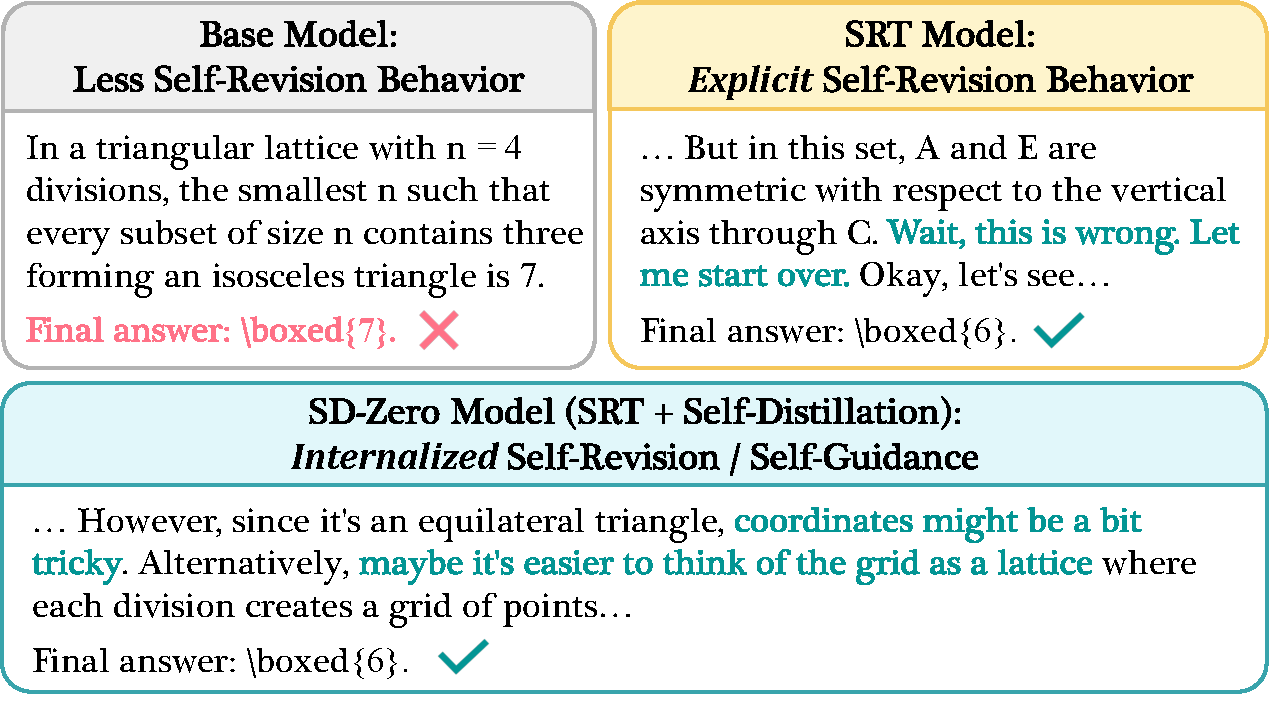
\includegraphics[width=\textwidth]{figures/Picture3.pdf}
    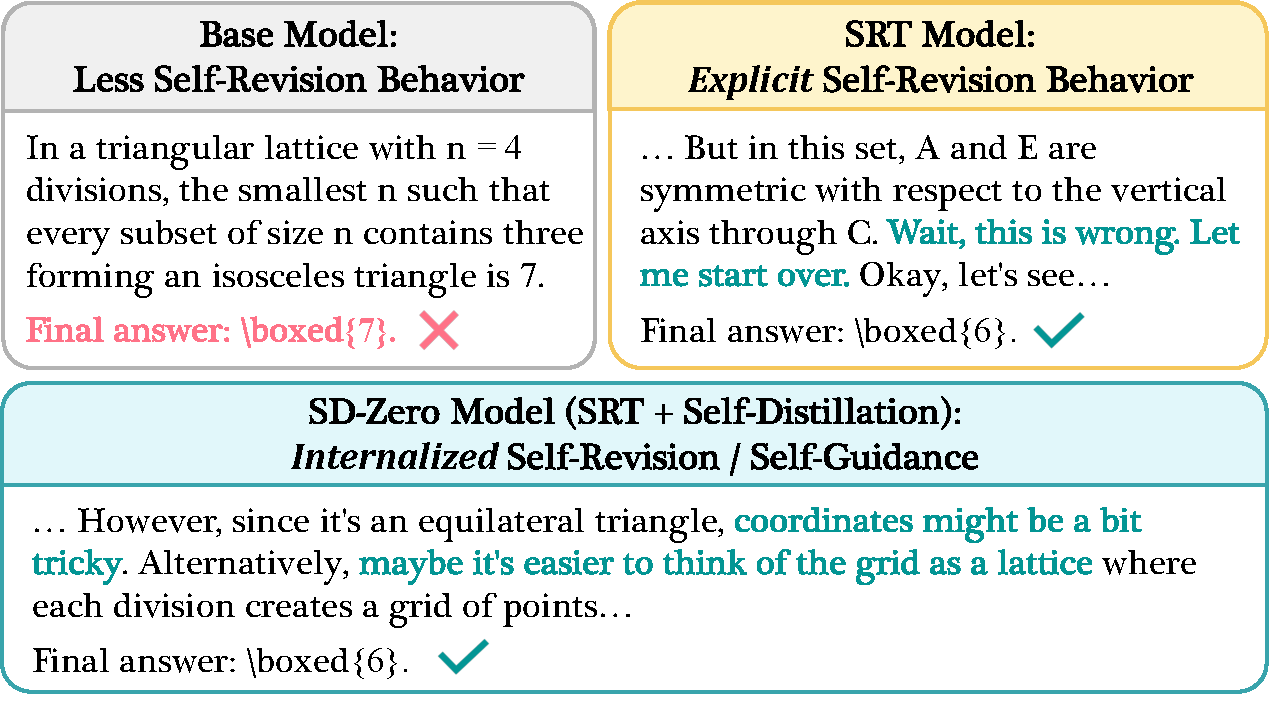
\includegraphics[width=0.57\textwidth]{figures/Picture3.pdf}
    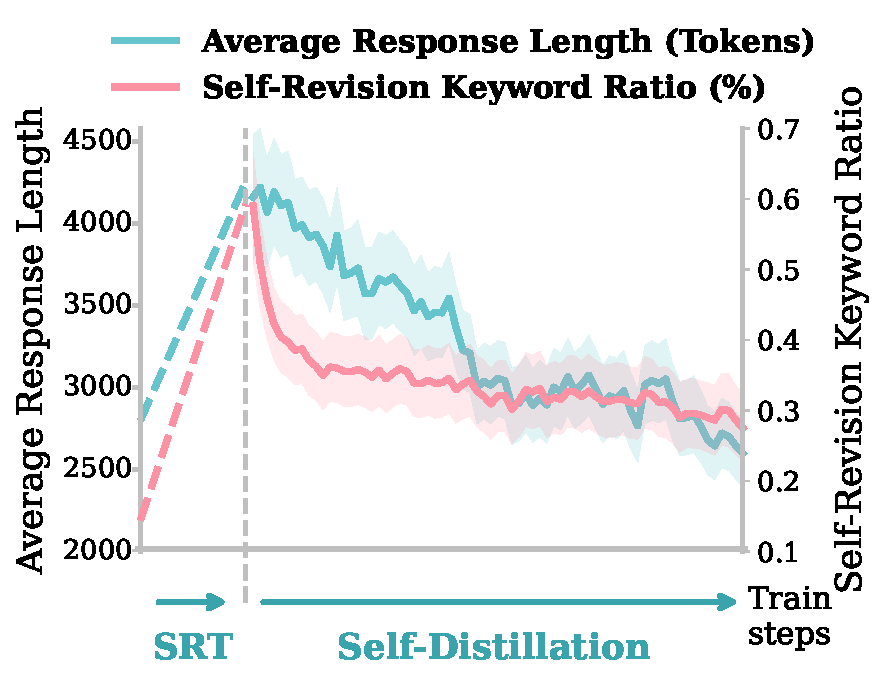
\includegraphics[width=0.42\textwidth,
    trim=0cm 0.1cm 0.1cm 0.4cm,
    clip
    ]{figures/publication_plot.pdf}
    \vspace{-1em}
    \captionsetup{font=small}
    \caption{\textbf{Evolution of self-revision behavior across training phases} for \qwen{} on \openmath{}. \textbf{Left:} Example reasoning traces from different model phases. The base model fails without revision, whereas the \sft{} model performs explicit self-revision and the \ours{} model exhibits more internalized self-guidance, identifying pitfalls and directing itself to the correct answer. \textbf{Right:} Training dynamics of self-revision behavior. Response length and explicit self-revision keywords rise during the SRT phase and fall during the \opsd{} phase, indicating a shift from overt revision to more internalized, token-efficient reasoning.}
    % \vspace{-10pt}
    \label{fig:behavior-evolution}
\end{figure}

% \subsection{Evolution of Reasoning Behaviors in \ours{} Training}\label{sec:behavioral_analysis}
\subsection{Evolution of Reasoning Behaviors: \ours{} Internalizes Self-Revision}\label{sec:behavioral_analysis}
% \textbf{\ours{} Internalizes Verbatim Self-Revision into Proactive Reasoning.}
% \paragraph{Behavioral Analysis:} 
%Self-Distillation Internalizes Revision into Compact Reasoning
% The accuracy gains in the previous section raise a natural question: does self-distillation simply improve performance, or does it change \emph{how} the model reasons? We find evidence for the latter.
% We study how the model's generation behavior changes over the course of training in \ours{}.

\looseness-1As shown in \Cref{fig:self-revision}, the \ours{} model after \opsd{} training produces substantially shorter generations, suggesting that it might have internalized some
formerly explicit reasoning. Here, we take a closer look at how this generation behavior evolves over \ours{} training.
Figure~\ref{fig:behavior-evolution} \text{(Right)} tracks two statistics: average response length and frequency of explicit self-revision keywords (e.g., ``Wait'' ``let me start over''; see Appendix \ref{app:keywords} for the full keyword list). During the \sft{} phase, both metrics rise substantially. The model learns to solve problems by actively judging its own response and applying self-correction. During \opsd{} phase, the trend reverses: both response length and self-revision keyword frequency fall steadily, while accuracy continues to improve. The resulting model only uses approximately half as many tokens as the \sft{} model at better accuracy.

\looseness-1We qualitatively illustrate this two-stage pattern via example traces from different models in \Cref{fig:behavior-evolution} (Left). The base model answers with a false claim. The \sft{} model reached the correct answer by backtracking with the exact transition phrase seen in training (``Wait, this is wrong. Let me start over.’’). By contrast, the \ours{} model, without any backtracking, anticipates the same pitfall and directs proactively to the correct answer.
% The qualitative shift is visible in individual traces (Figure~\ref{fig:behavior-evolution} (Left)). 
% While the \sft{} model backtracks with verbatim transition keywords from the training data (``Wait, this is wrong. Let me start over.''), the \ours{} model anticipates the same pitfall and redirects proactively (``coordinates might be a bit tricky. Alternatively, maybe it's easier to think of the grid as a lattice''). 
Note that \opsd{} does not reduce the revision capability acquired in \sft{}. The model still achieves a 5.3\% gain in the Generate-then-Revise evaluation (Figure~\ref{fig:self-revision}), but it has successfully internalized some of that capability into a more directed, pitfall-aware attempt.

\subsection{Ablations on \ours{} Design}
\label{sec:ablations}

We examine several design choices in \ours{}.
% \textbf{Replacing Binary Reward with Self-Verification.} 

\looseness-1\textbf{Loss Terms in \sft{} Objective.} We ablate the two terms in \lsrt{} by training with only \lgen{} or only \lrev{} (\Cref{tab:phase1-ablation}). Neither alone matches full \sft{}: \lgen{} preserves stronger generation but weak self-revision, while \lrev{} improves revision but barely boosts generation. The two terms are therefore complementary: \lrev{} elicits self-revision, and \lgen{} transfers it to stronger generation.
% The SRT objective \lsrt{} (Section~\ref{sec:method}) combines two terms: the first term \lrev{} trains the model to produce a revision or rephrase conditioned on the outcome; the second term \lgen{} trains it to generate better responses by actively evaluating its current response and self-correcting. We ablate this by training with each term alone. If the self-correction term is redundant, removing it should not hurt Phase~2 performance; if the conditioned revision term is redundant, the model should still learn to revise from the self-correction objective alone. \yh{compare with SRT performance and figure 3}


\looseness-1\textbf{\opsd{} Phase without \sft{}.} \ours{} requires the model to have certain self-revision ability, which is unlocked only after the \sft{} phase (\Cref{fig:self-revision}). To further demonstrate its necessity, we apply the \opsd{} phase directly to \qwen{} without prior self-revision training. \Cref{tab:phase2-ablation} shows that this Phase-2-only variant yields only marginal improvements over the base model, and does not improve self-revision ability. Therefore, the \sft{} phase is necessary for \ours{} to be effective.

\looseness-1\textbf{Data Split Between Phases.} We study how to allocate a fixed training data budget between the \sft{} and \opsd{} phases. As shown in \Cref{tab:data-split-ablation}, giving more data to \sft{} slightly improves the \sft{} model, but does not improve the final performance. Instead, the best result is obtained by assigning more data to the \opsd{} phase, suggesting that once \sft{} has unlocked self-revision capability, \opsd{} phase uses additional data more effectively to distill and refine this behavior into stronger generation.

% Allocating more data to SRT yields a stronger reviser but leaves fewer examples for distillation; conversely, too little SRT data may produce a reviser too weak to provide useful token-level supervision. We expect a non-monotonic relationship: at one extreme, insufficient SRT data yields a weak reviser whose noisy supervision limits Phase~2; at the other, over-allocating to SRT starves Phase~2 of fresh examples. We vary the split across \sk{todo: insert} to identify the tradeoff.


%\section{Discussion (Alt version)}

%\clearpage